\documentclass[oneside]{book}
\usepackage{epsfig,graphicx} % Required for inserting images
\usepackage{amsmath}
\usepackage{amsthm}
\usepackage{amssymb}
\usepackage{subcaption}
\usepackage[spanish,mexico]{babel}
\usepackage[bookmarksopen]{hyperref}
\usepackage[utf8]{inputenc}
\usepackage{array}
\usepackage{listings} %Soporte para código
\usepackage[left=2cm,right=2cm,top=1.8cm,bottom=2.3cm]{geometry}
\usepackage{titlesec}
\usepackage{fancyhdr} 
\usepackage{enumitem}
\usepackage{multicol}           % Permits header customization. See header section below.
\usepackage{wrapfig}
% ---definición de los paquetes--

\fancypagestyle{plain}{
    \lhead{}
    \fancyhead[R]{\thepage}
    \fancyhead[L]{}
    \renewcommand{\headrulewidth}{0pt}
    \fancyfoot{}
}
\pagestyle{fancy}
\fancyhead[R]{\thepage}
\fancyhead[L]{}
% Definir el tamaño del título del capítulo
\titleformat{\chapter}[display]
  {\normalfont\huge\bfseries} % Estilo del título
  {\chaptertitlename\ \thechapter}{1pt}{\Large} % Tamaño del título
  \titlespacing*{\chapter}{0pt}{-20pt}{20pt} % Ajustar el espaciado

\title{2da lista de problemas}
\author{Ramírez Mendoza Joaquín Rodrigo\\
Villalobos Juárez Gontran Eliut\\
Treviño Puebla Héctor Jerome}
\date{\today}
% ---Inicio de la portada
\begin{document}
\begin{titlepage}

	\begin{minipage}{3cm}
		\begin{center}
			
\includegraphics[height = 0.14\textheight]{recursos/Logo_UNAM.png}\par
		\end{center}
	\end{minipage}\hfill
	\begin{minipage}{10cm}

	\end{minipage}\hfill
	\begin{minipage}{3cm}
		\begin{center}
			
\includegraphics[height = 0.14\textheight]{recursos/Logo_FC.png}\par
		\end{center}
	\end{minipage}
	\centering
	\vspace{1cm}

	{\bfseries\LARGE Universidad Nacional Autónoma de México \par}

	\vspace{1cm}
	{\scshape\Large Facultad de Ciencias \par}
	\vspace{1cm}
	{\scshape\Large Matemáticas para las Ciencias Aplicadas 1 \par}
	\vspace{1cm}
	{\scshape\Large Licenciatura en Ciencias de la Computación \par}
	\vspace{1cm}
	{\scshape\Huge 2da lista de problemas  \par}
	\vspace{3cm}
	{\itshape\Large Segundo Parcial \par}
	\vfill
	{\Large Autores: \par}
	{\Large Ramírez Mendoza Joaquín Rodrigo \par}
	{\Large Villalobos Juárez Gontran Eliut\par}
	{\Large Treviño Puebla Héctor Jerome \par}
	\vfill
	{\Large Septiembre 2024 \par}
\end{titlepage}
% ---Fin de la portada de la portada
\maketitle

% Introducir aquí sus capítulos
\chapter*{CONSTRUCCIÓN DE UNA MONTAÑA RUSA}

\textbf{1)} Suponga que se le solicita diseñar el primer ascenso y descenso de un nuevo modelo de cohete. Después de estudiar fotografías de sus momentos rusos y precedentes, decide hacer la pendiente de ascenso 0.8 y la de descenso -1.6. Opta por conectar estos dos tramos rectos y es \( L(x) \) en pies para el tramo que parte del suelo y es \( f(x)= ax^2 + bx + c \), donde \( f'(x) \), su derivada, es \( 2ax + b \). Mediante el trabajo ya mencionado, puede calcular ambos coeficientes de dirección por lo que dispone que los segmentos para \( L \) y \( S \), sean tangentes al parabola en los puntos P y Q. Para simplificar las ecuaciones, decide situar el origen en P.

\begin{enumerate}[label=\alph*)]
	\item Suponga que la distancia horizontal entre P y Q es 100 pies. Escriba ecuaciones en \( a \), \( b \) y \( c \) que aseguren que le trayecto sea suave en los puntos de transición.
	\item Resuelva las ecuaciones del Inciso a) para \( a \), \( b \) y \( c \) para hallar una fórmula para \( f(x) \).
	\item Dibuje \( L_1 \) y \( L_2 \) para verificar gráficamente que las transiciones sean suaves.
	\item Encuentre la diferencia en elevación entre P y Q.
\end{enumerate}

\textbf{Inciso a)} Sea la coordenada \textbf{P} en el origen ya que es un punto conocido

$\therefore$ para la ecuación de la curva $f(x)$ pasa por el origen en el punto \textbf{P}, entonces $f(0)=0=a(0)^2 + b(0) + c \therefore c=0$

La derivada retorna la pendiente de la recta tangente en un punto de la curva y sabemos que el valor de la pendiente en el punto $P = 0.8$, por tanto:
\begin{align*}
	f'(x)|_{P(0,y)}=2ax+b|_{P(0,0)}=2a(0)+b=0.8 \\
	\therefore b=0.8
\end{align*}
Aplicando la misma lógica para el punto $Q(100,y(100))$ donde la pendiente $m_2=-1.6$:
\begin{align*}
	f'(x)|_{Q(100,y)}=2ax+b|_{Q(100,y)}=2a(100)+b= & -1.6 \\
	\implies 2(100)a+b=                            & -1.6 \\
	\therefore 200a+b=                             & -1.6 \\
\end{align*}

\textbf{Inciso b)} Hallar la fórmula f(x) resolviendo para a, b y c.
Por el inciso anterior sabemos que $b=0.8$ y $c=0$, entonces
\begin{align*}
	200a+0.8 & =-1.6             \\
	200a     & =-1.6-0.8         \\
	a        & =\frac{-2.4}{200} \\
	a        & =-0.012           \\
\end{align*}
$\therefore f(x)=-0.012x^2+0.8x$\\
$f'(x)=-0.024x+0.8$
\vspace*{1em}
\\
\textbf{Inciso c)} Dibular $L_1$ y $L_2$

Para dibujar las rectas neceistamos la derivada de la función $f(x)$, además sabemos que las ecuaciones de las rectas tangentes a cada punto de definen de la forma $y=(y(x_0)+y'(x_0)(x-x_0))$ para $L_1$ y $L_2$.

\begin{multicols}{2}
	\noindent
	\begin{align*}
		L_1= & (y(P_x)+y'(P_x)(x-P_x)), \;P(0,0) \\
		L_1= & 0+0.8(x-0)                        \\
		L_1= & 0.8x
	\end{align*}
	\columnbreak
	\begin{align*}
		L_2= & (y(Q_x)+y'(Q_x)(x-Q_x)), \;Q(100,y(100)) \\
		L_2= & -40-1.6(x-100)                           \\
		L_2= & -40-1.6x+160                             \\
		L_2= & 120-1.6x                                 \\
	\end{align*}
\end{multicols}

\begin{center}
	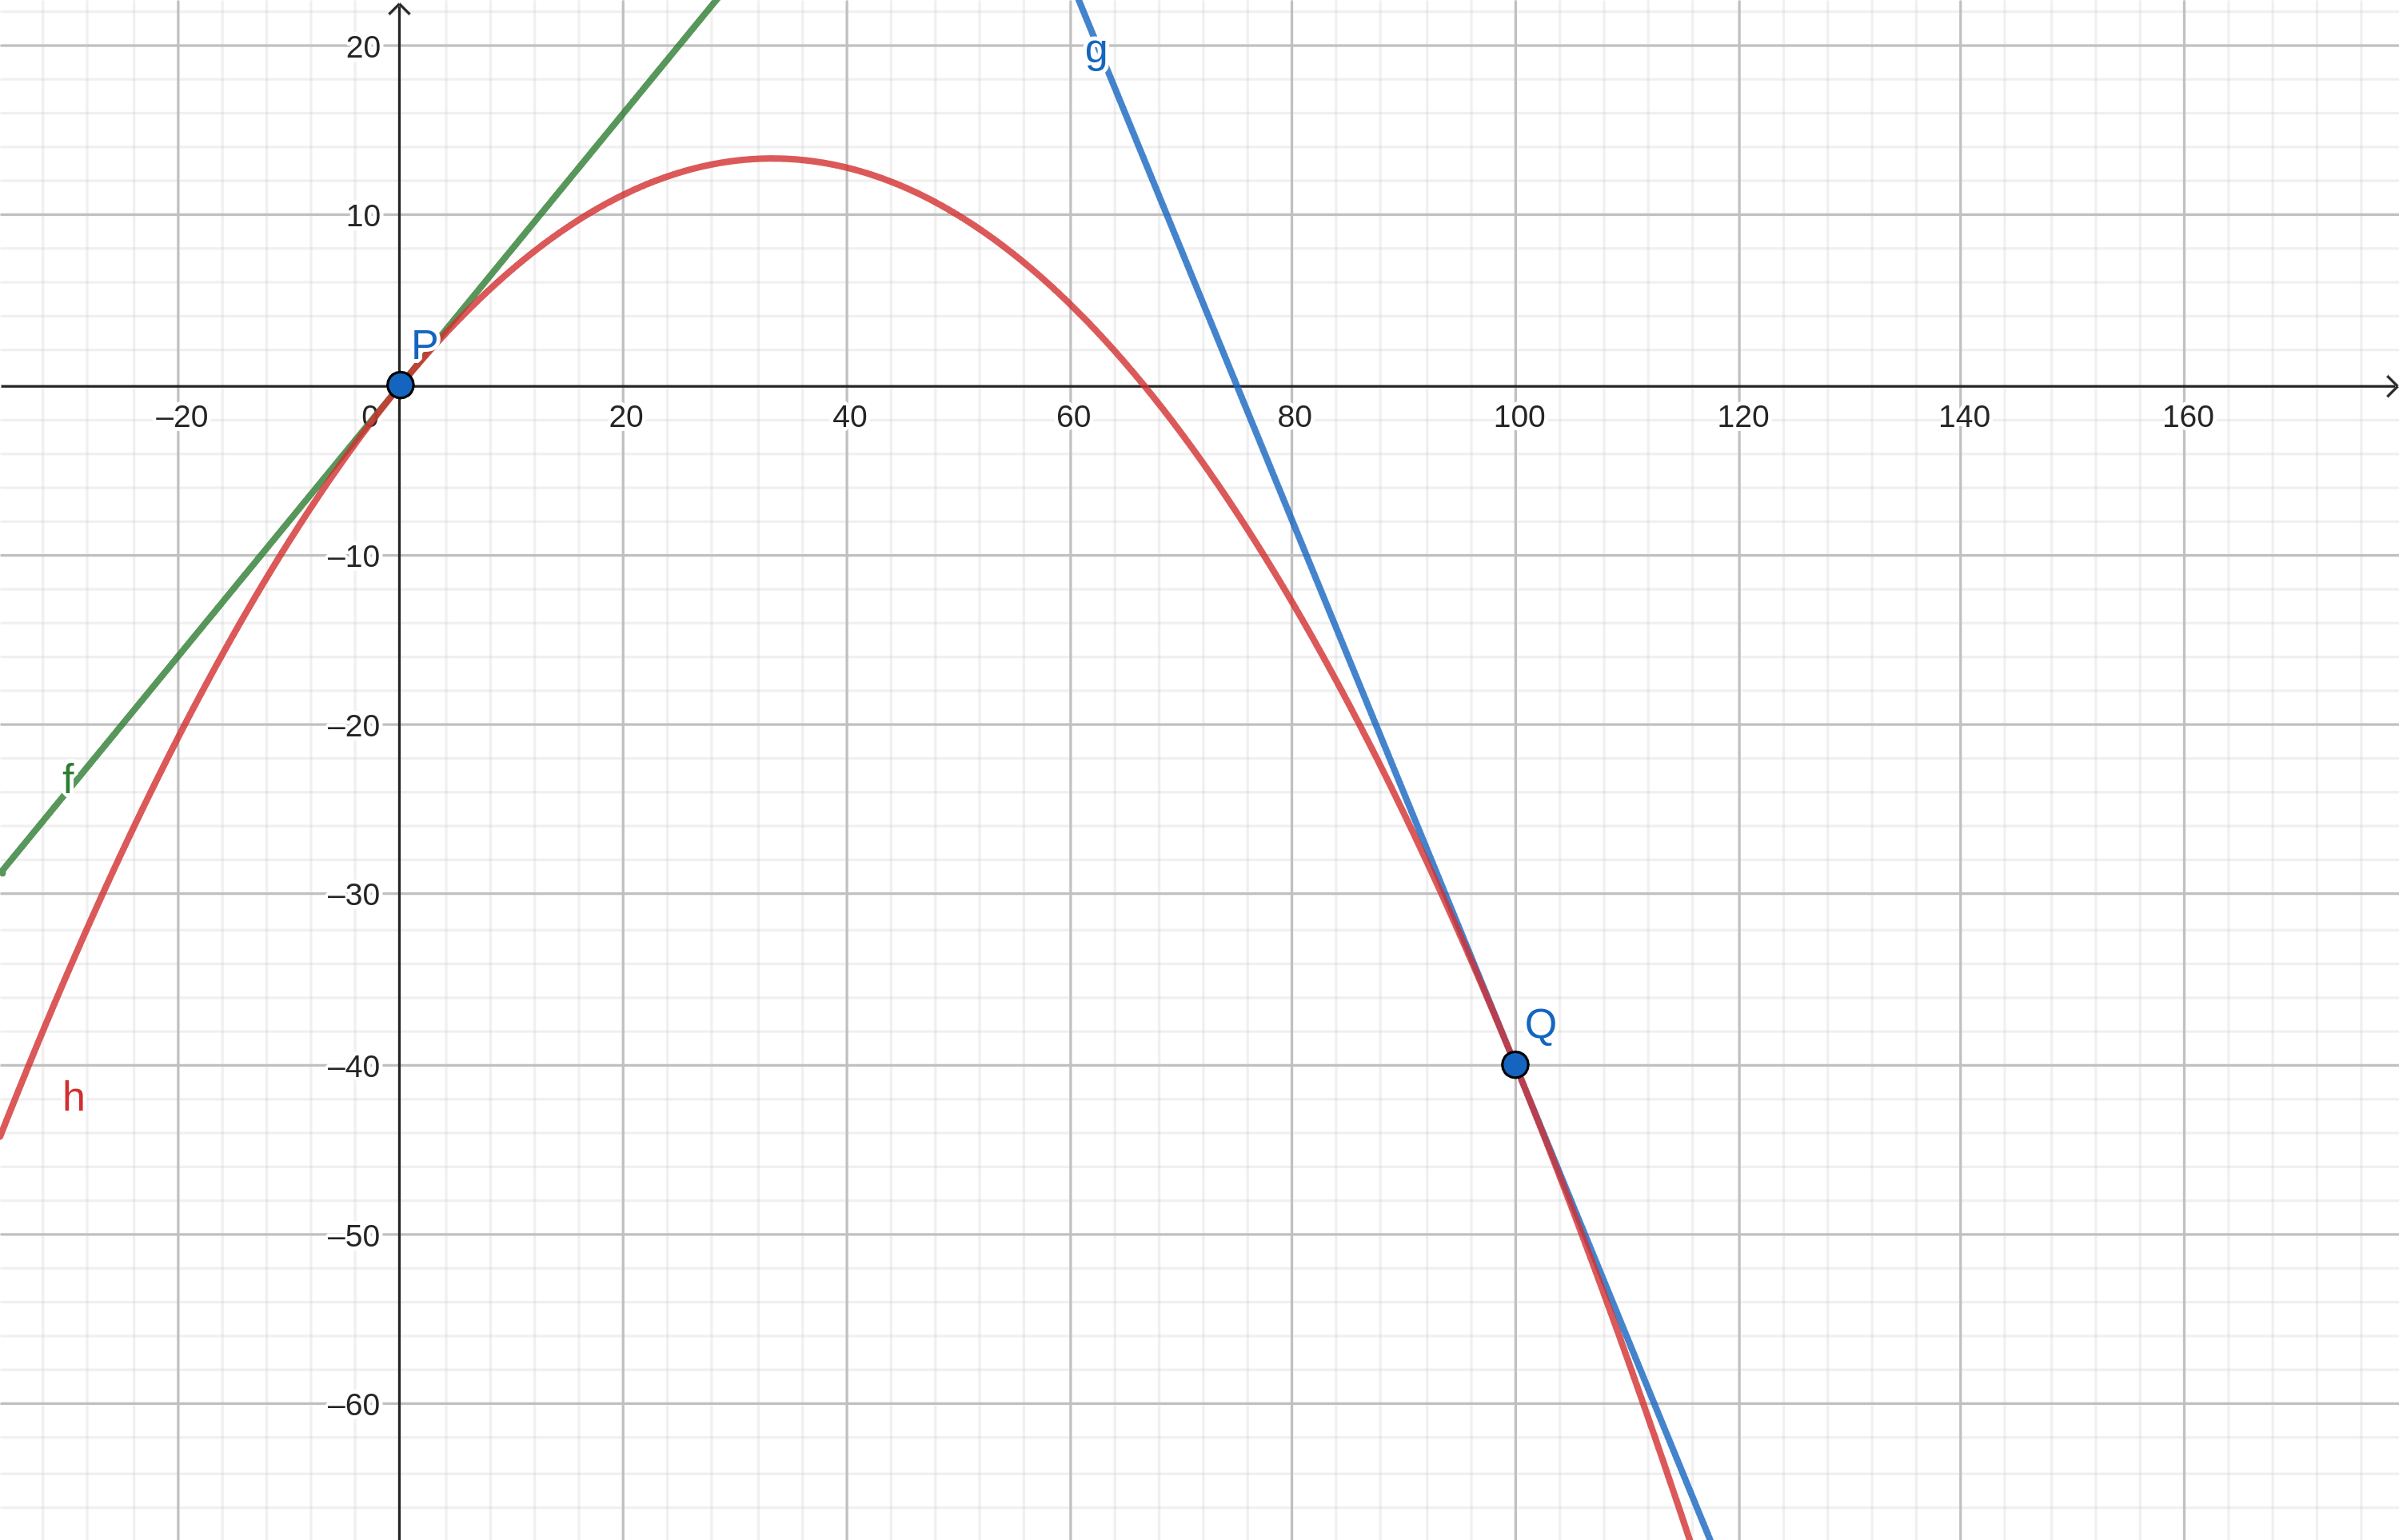
\includegraphics[height = 0.3\textheight]{recursos/geogebra-export.png}\par
\end{center}

\textbf{Inciso d)} La diferencia de elevación de cada punto está dado por el valor absoluto de la diferencia con respecto a el eje cordenado $y$ de los dos puntos

\begin{multicols}{2}
	\noindent
	\begin{align*}
		\text{Para el punto P} \\
		f(0)=0                 \\
	\end{align*}
	\columnbreak
	\begin{align*}
		\text{Para el }  & \text{punto Q en}  x = 100 \\
		f(100)           & =-0.012(100)^2+0.8(100)    \\
		f(100)           & =-0.012(100)^2+0.8(100)    \\
		f(100)           & =-120+80                   \\
		f(100)           & =-40                       \\
		\therefore Q(100 & ,-40)
	\end{align*}
\end{multicols}

$$\implies diferencia = |0-40|=40ft$$
\newpage
\textbf{2)} La solución del problema 1 puede parecer suave, pero es posible que no sienta lo suave debido a que la pieza definida como función [consistente en $L_1(x)$ para $x < 0$, $f (x)$ para $0 \leq x \leq 100$; y $L_2(x)$ para $x > 100$] no tiene una segunda derivada continua. Por consiguiente, usted decide mejorar su diseño utilizando una función cuadrática $q(x) = ax^2 + bx + c$ únicamente en el intervalo $10 \leq x \leq 90$ y conectarlo con las funciones lineales por medio de dos funciones cúbicas:
\begin{align*}
	g(x) & = kx^3 + lx^2 + mx + n \quad 0 \leq x < 10   \\
	h(x) & = px^3 + qx^2 + rx + s \quad 90 < x \leq 100
\end{align*}

\begin{enumerate}[label=\alph*)]
	\item Escriba un sistema de ecuaciones con 11 incógnitas que aseguren que las funciones y sus derivadas sean continuas en los puntos de transición.

	\item Resuelva las derivadas implicadas en un sistema algebraico computarizado para encontrar las fórmulas para \( g(x) \), \( q(x) \), y \( h(x) \).

	\item Dibuje $L_1$, $g$, $q$, $h$ y $L_2$ y compárelas con las gráficas del problema 1 anexo.
\end{enumerate}

\textbf{Inciso a)} Tenemos las funciones defindas en los siguientes intervalos
\begin{table}[!hbt]
	\begin{center}
		\begin{tabular}{| l | l | l | l | }
			\hline
			Función                       & Primera Derivada         & Segunda derivada & Intervalo       \\ \hline
			$L_1(x)=0.8x$                 & $L_1'(x)=0.8$            & $L_1 ''(x)=0$    & $(-\infty,0)$   \\
			$g(x) = kx^3 + lx^2 + mx + n$ & $g'(x) =3kx^2 + 2lx + m$ & $g''(x)=6kx+2l$  & $[0,10)$        \\
			$q(x) = ax^2 + bx + c$        & $q'(x) =2ax + b$         & $q''(x)=2a$      & $[10,90]$       \\
			$h(x) = px^3 + qx^2 + rx + s$ & $h'(x) =3px^2 + 2qx + r$ & $h''(x)=6px+2q$  & $(90,100]$      \\
			$L_2(x) = 120-1.6x$           & $L_2'(x)=-1.6$           & $L_2''(x)=0$     & $[100, \infty)$ \\ \hline
		\end{tabular}
		\caption{Tabla de funciones}
		\label{tab:la suma de los cilindros circunscritos como parabola}
	\end{center}
\end{table}

De acuderdo con lo establecido, las diferentes funciones deben ser iguales en los puntos de transición para garantizar que la entrada a la curva sea suave.

\begin{multicols}{4}
	\noindent
	\begin{align*}
		\text{Para } x = & 0        \\
		g(0)  =          & L_1(0)   \\
		g'(0) =          & L_1'(0)  \\
		g''(0)=          & L_1''(0) \\
	\end{align*}
	\columnbreak
	\begin{align*}
		\text{Para } x = & 10      \\
		g(10)  =         & q(10)   \\
		g'(10) =         & q'(10)  \\
		g''(10)=         & q''(10) \\
	\end{align*}
	\columnbreak
	\begin{align*}
		\text{Para } x = & 90       \\
		q(90)            & =h(90)   \\
		q'(90)           & =h'(90)  \\
		q''(90)          & =h''(90) \\
	\end{align*}
	\columnbreak
	\begin{align*}
		\text{Para } x = & 100        \\
		h(100)  =        & L_2(100)   \\
		h'(100) =        & L_2'(100)  \\
		h''(100)=        & L_2''(100) \\
	\end{align*}
\end{multicols}

Por lo tanto tenemos el siguiente sistema de ecuaciones de 11 incognitas.
\begin{align*}
	\text{Para }x=0                                      \\
	g(0)  = k(0)^3 + l(0)^2 + m(0) + n & = L_1(0)=0.8(0) \\
	g(0)  =  n                         & = L_1(0)=0      \\
	n                                  & = 0             \\
	g'(0) =3k(0)^2 + 2l(0) + m         & = L_1'(0)=0.8   \\
	g'(0) = m                          & = L_1'(0)=0.8   \\
	m                                  & = 0.8           \\
	g''(0)=6k(0)+2l                    & = L_1''(0)=0    \\
	g''(0)=2l                          & = L_1''(0)=0    \\
	2l                                 & = 0             \\
	l                                  & = 0             \\
	\therefore n=0; m=0.8; l=0                           \\
\end{align*}

\begin{align*}
	\text{Para }x=10                                                      \\
	g(10)  = k(10)^3 + l(10)^2 + m(10) + n & =q(10) = a(10)^2 + b(10) + c \\
	g(10)  = 1000k + 100l + 10m + n        & =q(10) = 100a + 10b + c      \\
	\implies 1000k + 100l + 10m + n        & =100a + 10b + c              \\
	g'(10) =3k(10)^2 + 2l(10) + m          & =q'(10) =2a(10) + b          \\
	g'(10) =3(100)k + 2(10)l + m           & =q'(10) =2(10)a + b          \\
	g'(10) =300k + 20l + m                 & =q'(10) =20a + b             \\
	\implies 300k + 20l + m                & =20a + b                     \\
	g''(10)=6k(10)+2l                      & =q''(10)=2a                  \\
	g''(10)=6(10)k+2l                      & =q''(10)=2a                  \\
	g''(10)=60k+2l                         & =q''(10)=2a                  \\
	\implies 60k+2l                        & =2a                          \\
\end{align*}
\begin{align*}
	\text{Para }x=90                                                     \\
	h(90) = p(90)^3 + q(90)^2 + r(90) + s & =q(90) = a(90)^2 + b(90) + c \\
	h(90) = 729000p + 8100q + 90r + s     & =q(90) = 8100a + 90b + c     \\
	\implies 729000p + 8100q + 90r + s    & = 8100a + 90b + c            \\
	h'(90) =3p(90)^2 + 2q(90) + r         & =q'(90) =2a(90) + b          \\
	h'(90) =3(8100)p + 2(90)q + r         & =q'(90) =2(90)a + b          \\
	h'(90) =24300p + 180q + r             & =q'(90) =180a + b            \\
	\implies 24300p + 180q + r            & =180a + b                    \\
	h''(90)=6p(90)+2q                     & =q''(90)=2a                  \\
	h''(90)=6(90)p+2q                     & =q''(90)=2a                  \\
	h''(90)=540p+2q                       & =q''(90)=2a                  \\
	\implies 540p+2q                      & =2a                          \\
\end{align*}

\begin{align*}
	\text{Para }x=100                                                    \\
	h(100) = p(100)^3 + q(100)^2 + r(100) + s & =L_2(100) = 120-1 6(100) \\
	h(100) = 1x10^6p + 1x10^4q + 100r + s     & =L_2(100) = 120-160      \\
	\implies 1x10^6p + 1x10^4q + 100r + s     & =-40                     \\
	h'(100) =3p(100)^2 + 2q(100) + r          & =L_2'(100)=-1.6          \\
	h'(100) =3(1x10^4)p + 200q + r            & =L_2'(100)=-1.6          \\
	\implies (3x10^4)p + 200q + r             & =-1.6                    \\
	h''(100)=6p(100)+2q                       & =L_2''(100)=0            \\
	h''(100)=600p+2q                          & =L_2''(100)=0            \\
	\implies 600p+2q                          & =0                       \\
\end{align*}

En resumen queremos resolver las ecuaciones para:
\begin{align*}
	n                                            & = 0   \\
	m                                            & = 0.8 \\
	2l                                           & = 0   \\
	-100a - 10b - c + 1000k + 100l + 10m + n     & =0    \\
	-20a - b +300k + 20l + m                     & = 0   \\
	- 2a + 60k+2l                                & =0    \\
	-8100a - 90b - c + 729000p + 8100q + 90r + s & = 0   \\
	-180a - b +24300p + 180q + r                 & = 0   \\
	1x10^6p + 1x10^4q + 100r + s                 & =-40  \\
	(3x10^4)p + 200q + r                         & =-1.6 \\
	600p+2q                                      & =0    \\
\end{align*}

\textbf{Inciso b)}Según el software \textbf{Matlab} el valor de cada incógnita es:
\begin{center}
	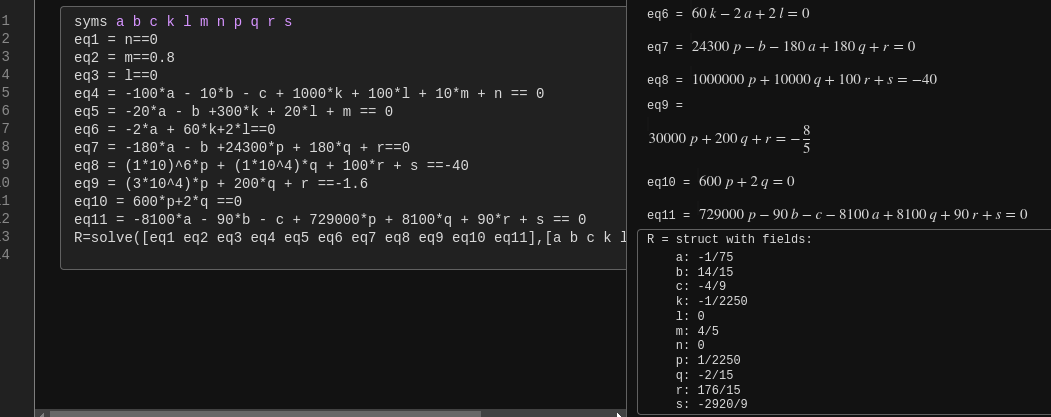
\includegraphics[height = 0.25\textheight]{recursos/Captura desde 2024-09-22 13-05-43.png}\par
\end{center}

$\implies$ Las formulas según los resultados son:
\begin{align}
	q(x) & =ax^2+bx+c                                   \\
	q(x) & =-\frac{1}{75}x^2+\frac{14}{15}x-\frac{4}{9}
\end{align}
\begin{align*}
	g(x) & =kx^3+lx^2+mx+n                         \\
	g(x) & =-\frac{1}{2250}x^3+0x^2+\frac{4}{5}x+0 \\
	g(x) & =-\frac{1}{2250}x^3+\frac{4}{5}x
\end{align*}
\begin{align*}
	h(x) & =px^3+qx^2+rx+s                                                   \\
	h(x) & =\frac{1}{2250}x^3-\frac{2}{15}x^2+\frac{176}{15}x-\frac{2920}{9} \\
\end{align*}

\textbf{Inciso c)} Las gráficas $L_1$, $g$, $q$, $h$ y $L_2$ y compárelas con las gráficas del problema 1 anexo.

\begin{figure*}
	\centering
	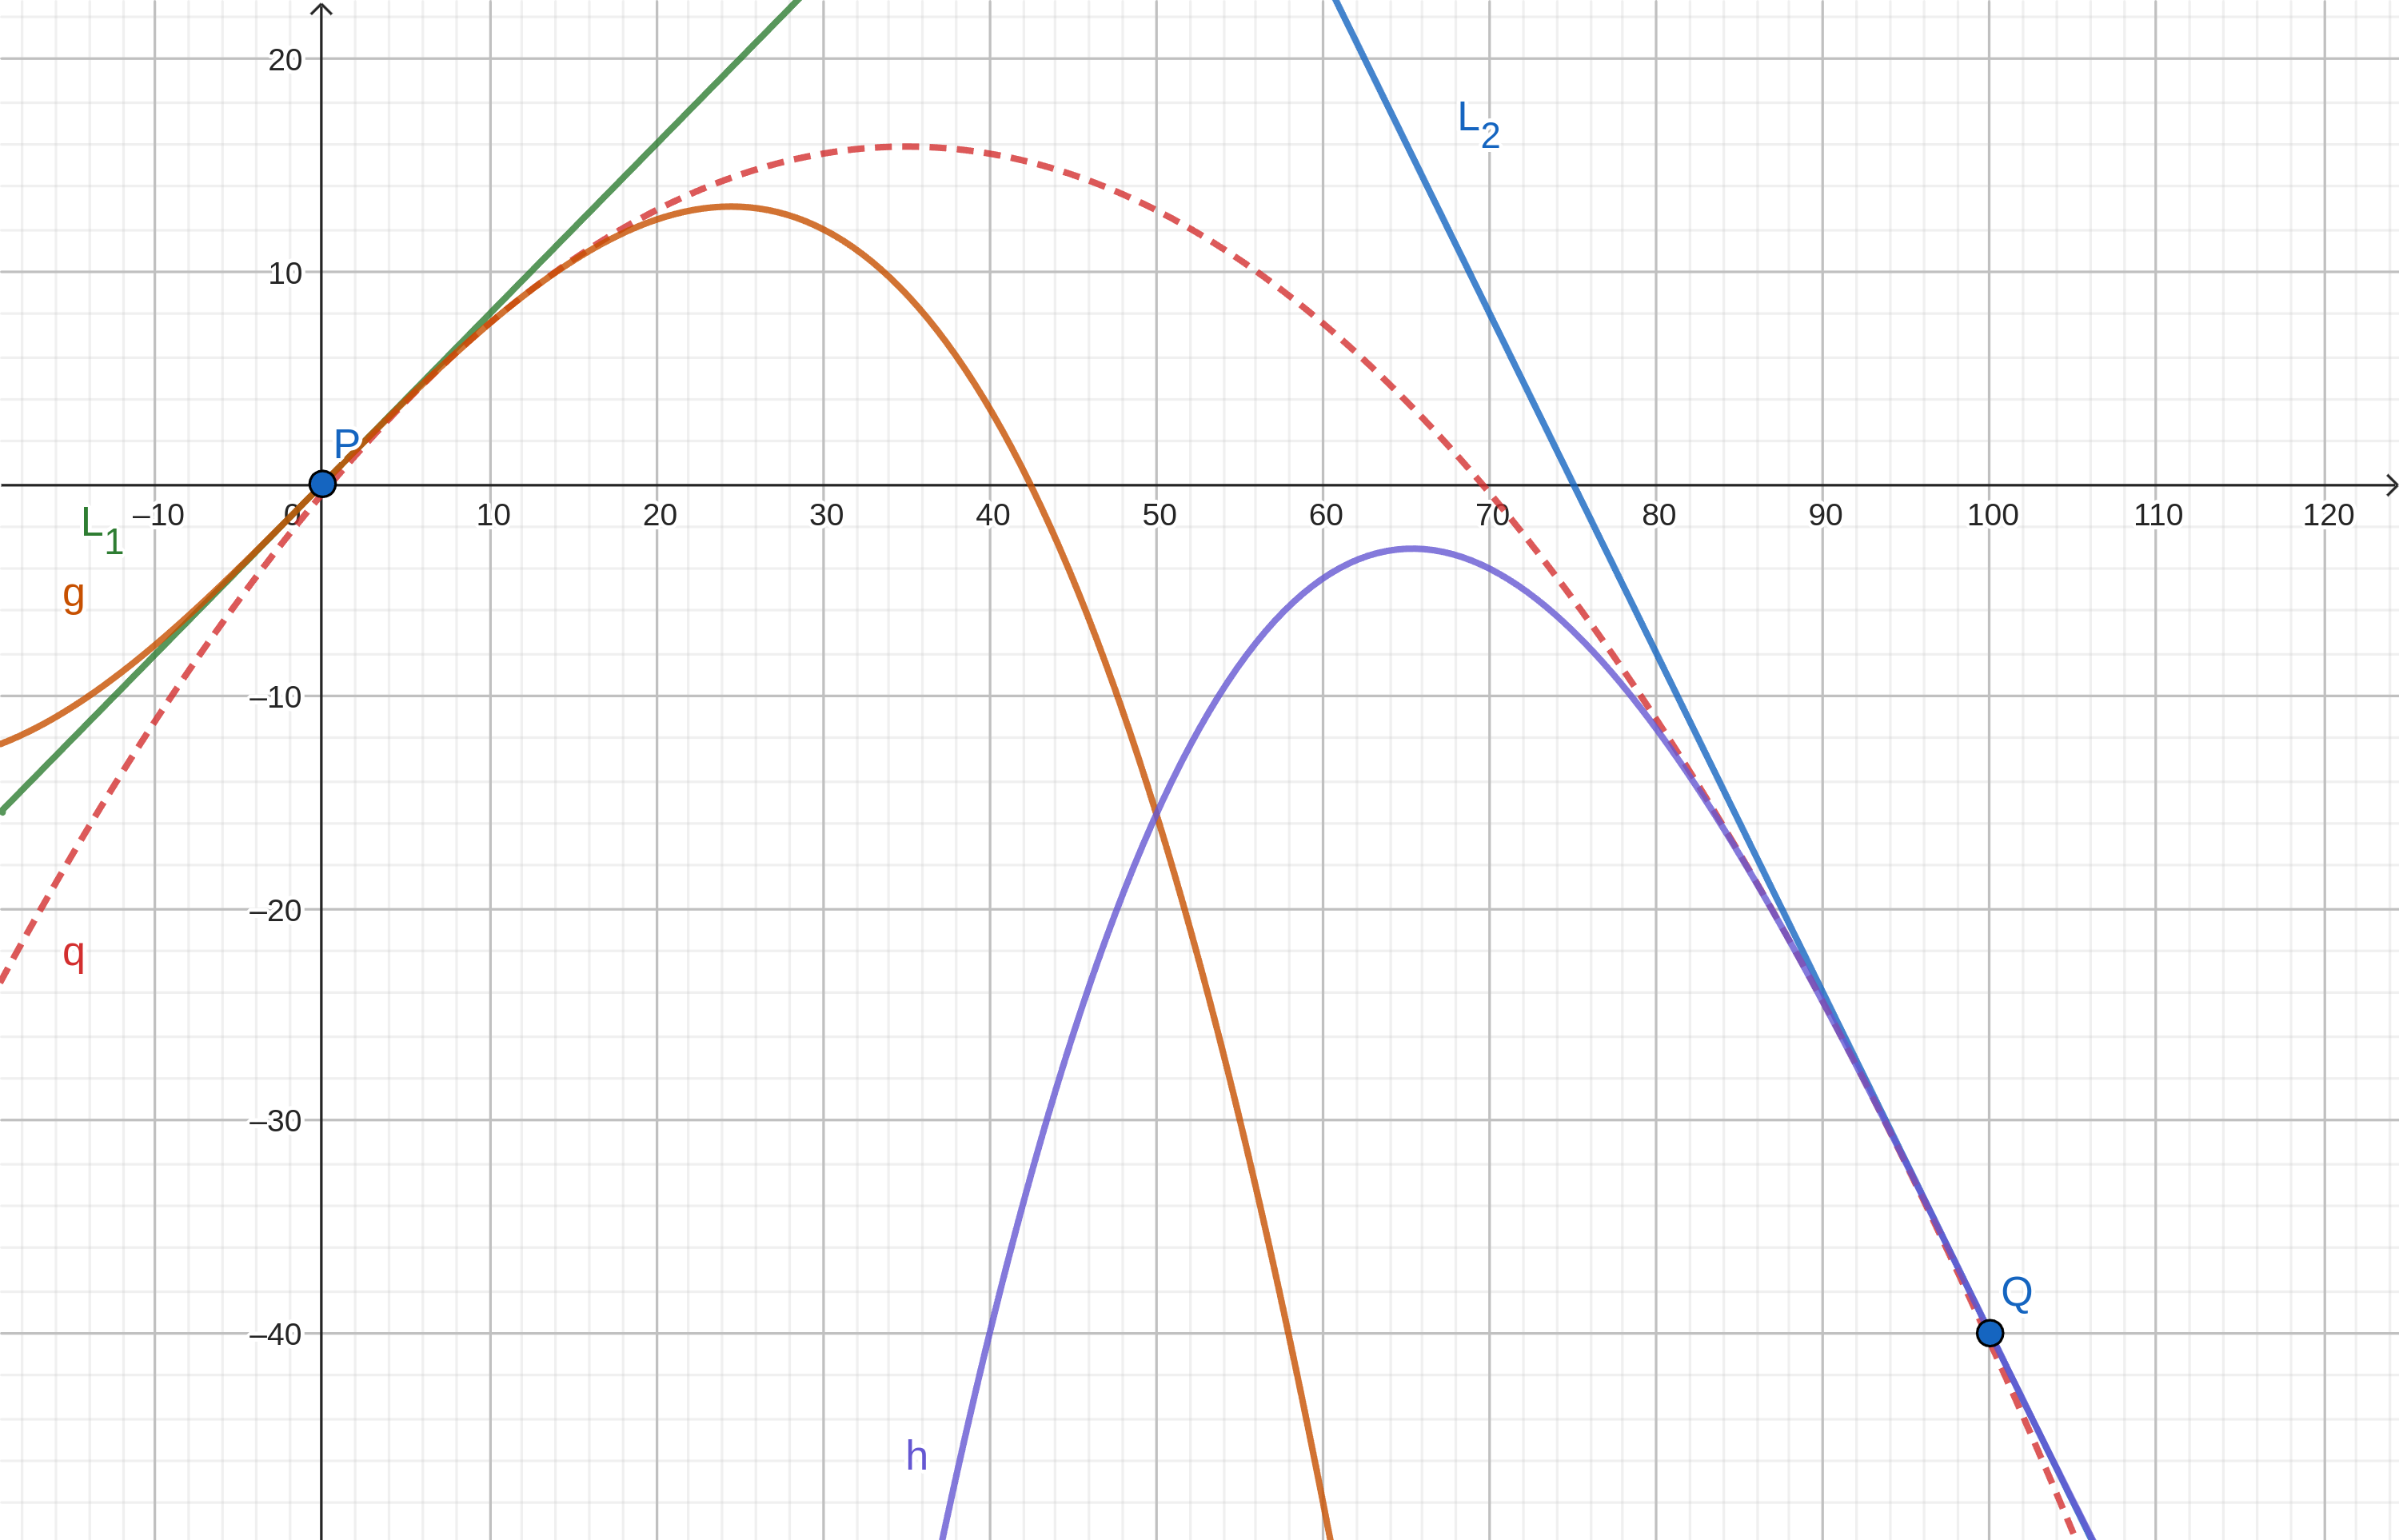
\includegraphics[height = 0.25\textheight]{recursos/geogebra-export1.png}\par
	\caption*{Las 5 ecuaciones completas que pasan por los mismos puntos de transición P y Q}
\end{figure*}

\begin{figure*}
	\centering
	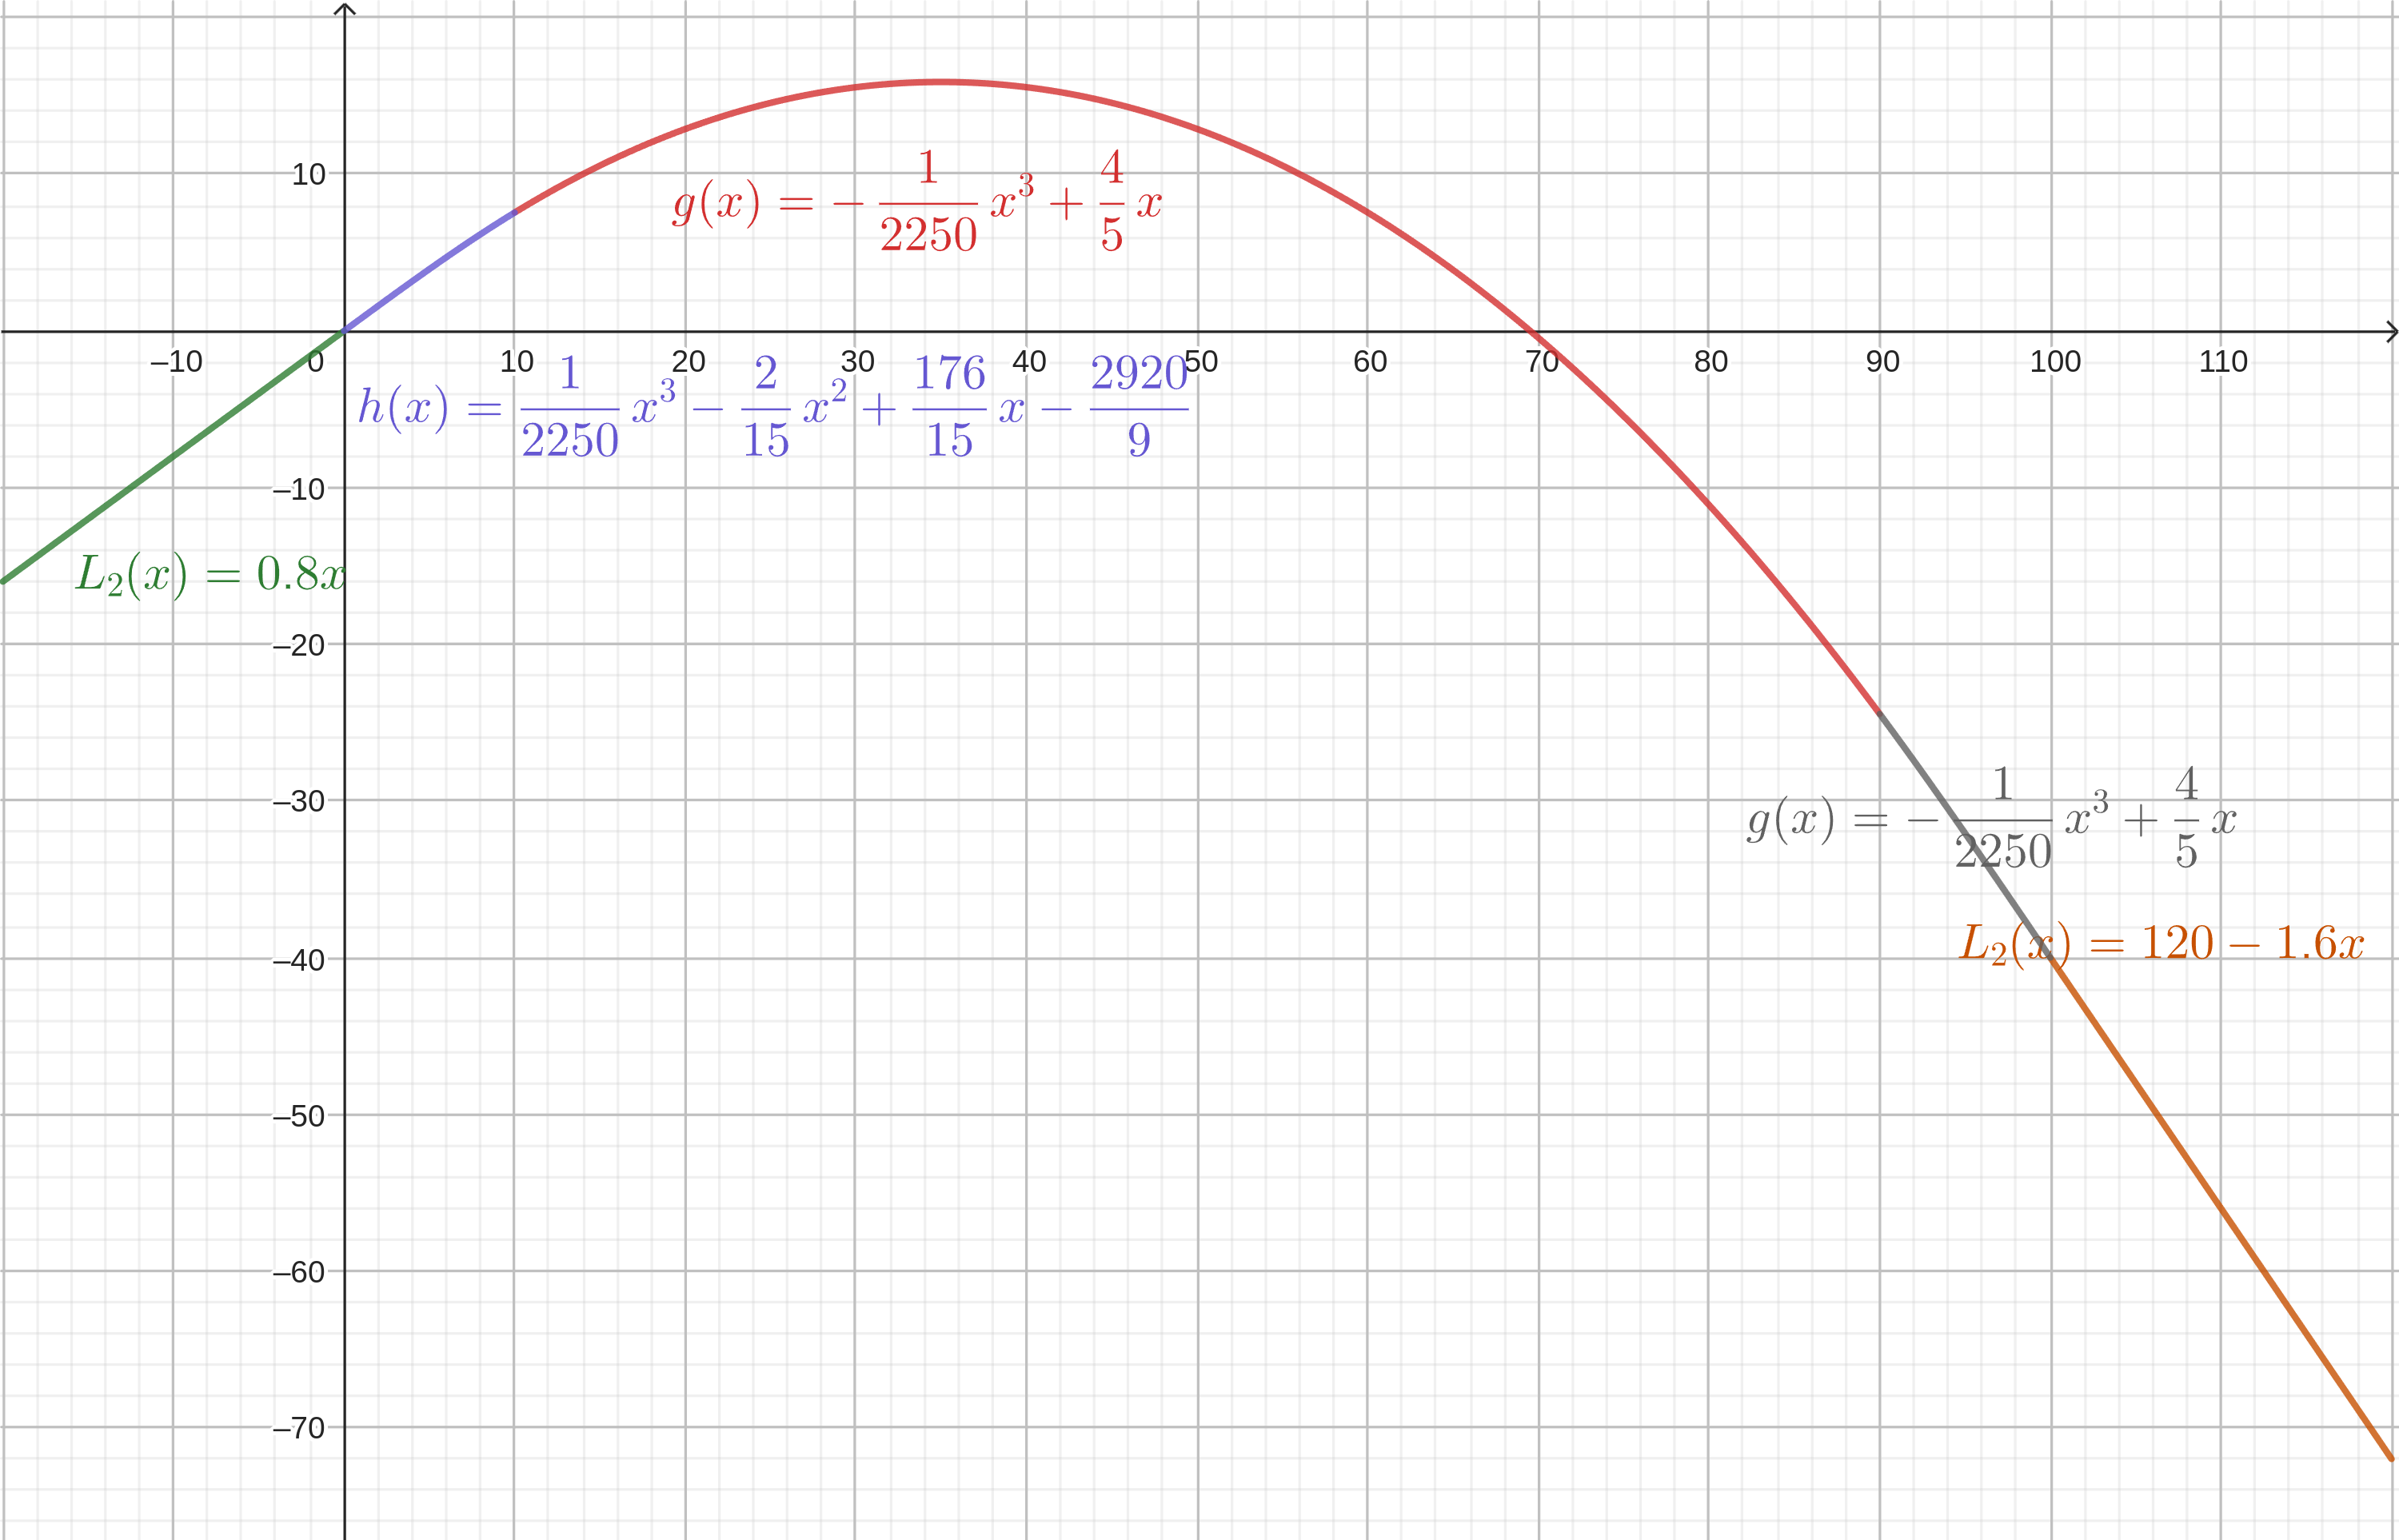
\includegraphics[height = 0.25\textheight]{recursos/geogebra-export2.png}\par
	\caption*{Las 5 ecuaciones de la parte dos del ejercicio con sus intervalos definidos para la construcción de la montaña Rusa.}
\end{figure*}
\begin{figure*}
	\centering
	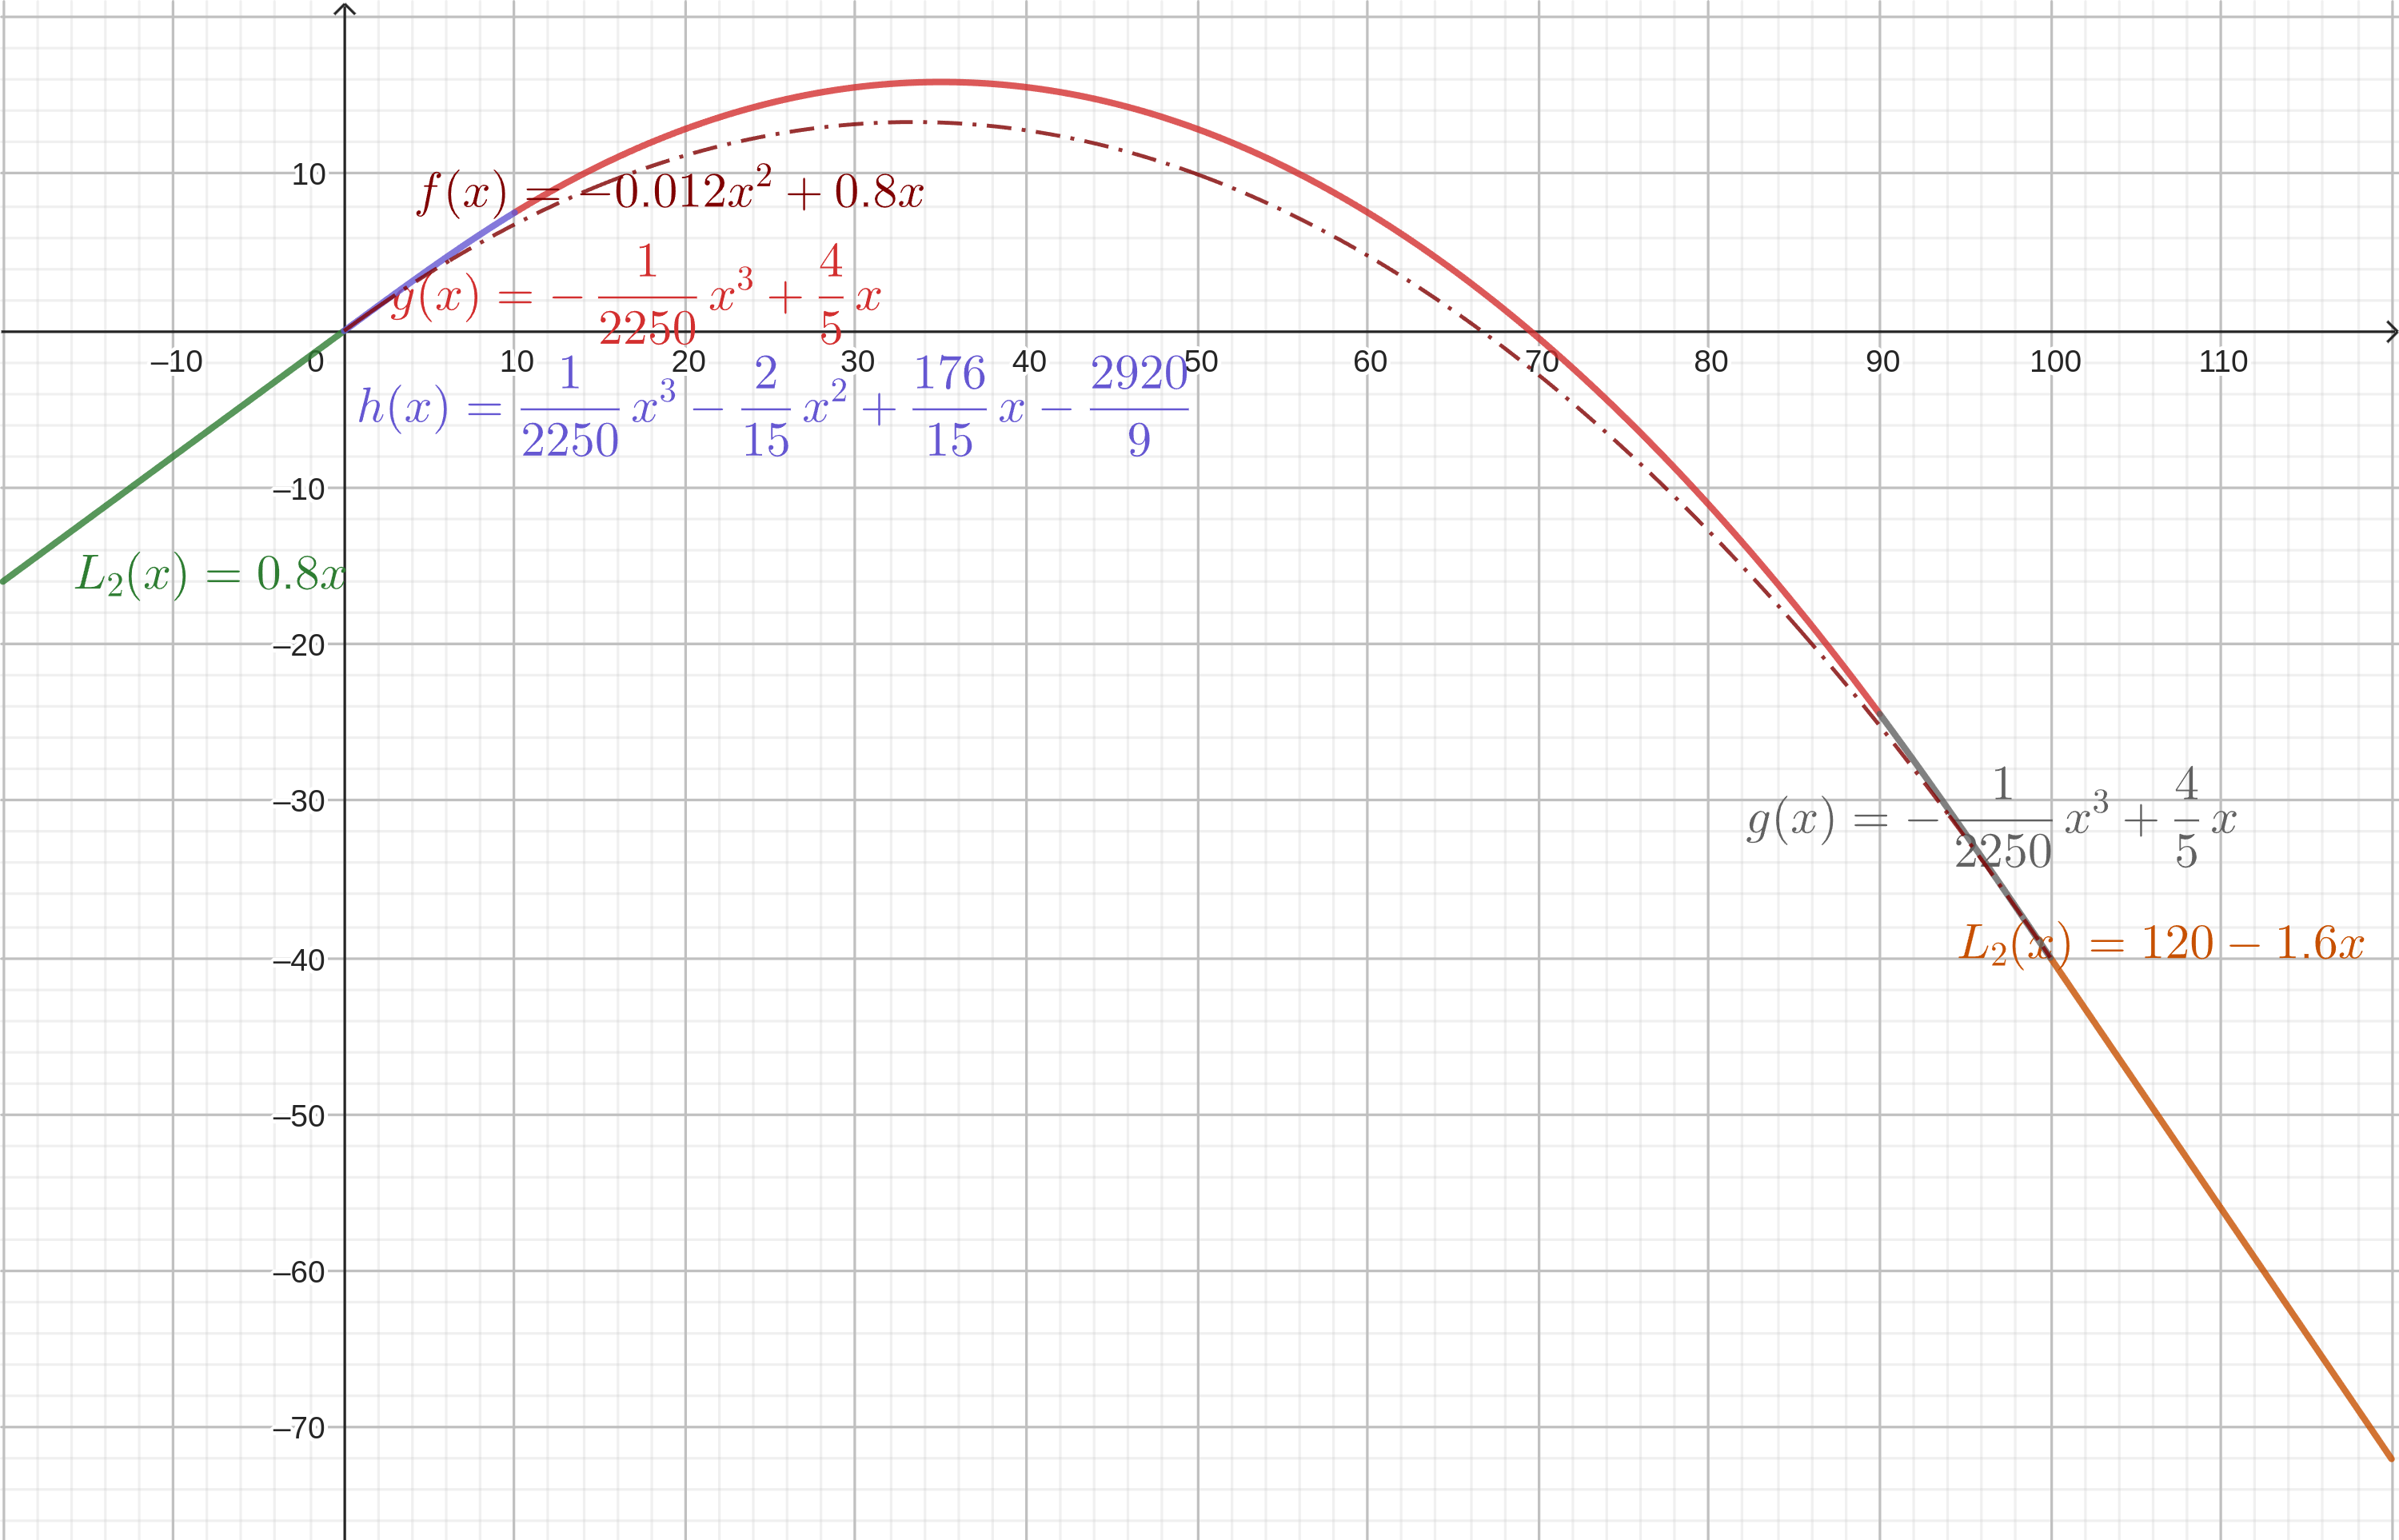
\includegraphics[height = 0.25\textheight]{recursos/geogebra-export3.png}\par
	\caption*{Comparación con la función generada en la primera parte del ejercicio mostrando, la segunda forma una continuidad más suave en cada transición}
\end{figure*}



\chapter*{¿Dónde debería un piloto iniciar su aterrizaje?}

\begin{wrapfigure}{l}{0.3\textwidth}
	\centering
	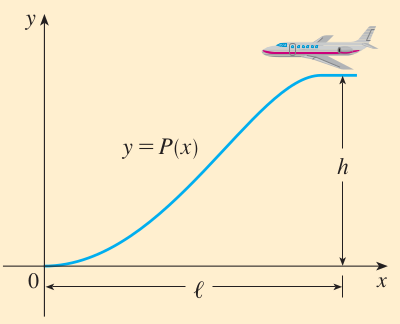
\includegraphics[width = 0.3\textwidth]{recursos/Captura desde 2024-09-21 16-53-03.png}
	\caption{caption}
	\vspace{-60px}
\end{wrapfigure}
En la figura se muestra una trayectoria de aproximación para el aterrizaje de un avión, que satisface las condiciones siguientes:

\begin{enumerate}[label=\Roman*)]
	\item La altura del crucero es $h$ cuando se inicia el descenso a una distancia $l$ del punto de contacto con la pista en el origen.
	\item El piloto debe mantener una rapidez horizontal constante $v$ a todo lo largo del descenso.
	\item El valor absoluto de la aceleración vertical no debe sobrepasar una constante $k$ (la cual es mucho menor que la aceleración debida a la gravedad).
\end{enumerate}

1. Encuentre un polinomio cúbico $P(x)= ax^3+ bx^2 + cx + d$ que satisfaga la condición I), imponiendo condiciones adecuadas sobre $P(x)$ y $P'(x)$ en el inicio del descenso y el contacto con la pista.

\vspace{10pt}

\noindent 2. Use las condiciones I) y III) para demostrar que$$\frac{6hv^2}{l^2}\leq k$$

\vspace{10pt}

\noindent 3. Suponga que una aerolínea comercial decide no permitir que la aceleración vertical de un avión sea mayor que $k = 860 mi/h^2$. Si la altitud de crucero de un avión es de $35 000$ pies y la rapidez de $300 mi/h$, ¿a qué distancia del aeropuerto debe el piloto iniciar el descenso?

\vspace{10pt}

\noindent 4.Trace la grafica de la trayectoria de aproximación si se satisfacen las condiciones que se enuncian en el problema 3.

\textbf{Inciso 1}.- Tenemos las condiciones
\begin{align*}
	P(l)  & =h                                                                       \\
	P(0)  & =0\text{ (Para un aterrizaje suave)}                                     \\
	P'(l) & =0\text{ (debido a que la pendiente en este punto es paralela al eje x)} \\
	P'(0) & =0                                                                       \\
\end{align*}
Primero debemos construir el polinomio de la forma $P(x)= ax^3+ bx^2 + cx + d$ donde su derivada es $P'(x)= 3ax^2+2bx +c$, usando las condiciones

\begin{multicols}{4}
	\noindent
	\begin{align*}
		P(l) & =h:                   \\
		     & al^3+ bl^2 + cl + d=h \\
	\end{align*}
	\columnbreak
	\begin{align*}
		P(0) & =0: \\
		d    & =0  \\
	\end{align*}
	\columnbreak
	\begin{align*}
		P'(l) & =0:            \\
		      & 3al^2+2bl +c=0 \\
	\end{align*}
	\columnbreak
	\begin{align*}
		P'(0) & =0: \\
		      & c=0 \\
	\end{align*}
\end{multicols}

$\implies$ Sustituimos $c$ y $d$ en las ecuaciones y decimos que $P(x)=ax^3+ bx^2 \text{ y } P'(l)= 3al^2+2bl$

Resolviendo para b:
$$b = -\frac{3al^2}{2l} = -\frac{3al}{2}$$
Sustituyendo de $P(l)=h$:
\begin{align*}
	al^3 - \frac{3al^2}{2}l           & = h               \\
	al^3 - \frac{3al^3}{2}            & = h               \\
	al^3 \left(1 - \frac{3}{2}\right) & = h               \\
	al^3 \left(-\frac{1}{2}\right)    & = h               \\
	\therefore a                      & = -\frac{2h}{l^3} \\
\end{align*}

Sustituyendo $a$ en $b$:
\begin{align*}
	a & = -\frac{2h}{l^3}                           \\
	b & = -\frac{3al}{2}                            \\
	  & = -\frac{3}{2}\left(-\frac{2h}{l^3}\right)l \\
	  & = \frac{3h}{l^2}
\end{align*}

Sutituimos la expresión anterior en $P(x)$
$$\implies P(x) = -\frac{2h}{l^3}x^3 + \frac{3h}{l^2}x^2$$

\textbf{Inciso 2}.- Demostrar que $\frac{6hv^2}{l^2} \leq k$

Por el inciso \textbf{II)} nos dice que la velocidad horizontal es constante, $x'(t)=-v, \forall t$ por lo que la posición $x$ en función del tiempo $t$ es: $l-v(t)$ donde $l$ es la distancia al punto de contacto con la pista cuando el descenso comienza, de este modo se asegura que en el transcurso del tiempo $t$ implicará que el crucero efectivamente recorrió la distancia requerida para llegar a la pista de aterrizaje en un tiempo $t$.

El inciso \textbf{III)} dice que el valor absoluto de la aceleración vertical no debe sobrepasar una constante $k$. Establece el límite en la aceleración vertical, por lo que, $\left|\frac{d^2 y}{dt}\right|\leq k$

Primero, calculamos la derivada primera de $y$ respecto a $x$ usando la regla de la cadena:
$$\frac{dy}{dt} = \frac{dy}{dx} \cdot \frac{dx}{dt}$$
Tenemos que $y = P(x) = -\frac{2h}{l^3} x^3 + \frac{3h}{l^2} x^2$, derivamos respecto a $x$
\begin{align*}
	\frac{dy}{dx} & = \frac{d}{dx} \left(-\frac{2h}{l^3} x^3 + \frac{3h}{l^2} x^2 \right) \\
	              & = -\frac{6h}{l^3} x^2 + \frac{6h}{l^2} x
\end{align*}

Dado que tenemos que $\frac{dy}{dt} = \frac{dy}{dx} \cdot \frac{dx}{dt}$ y $\frac{dx}{dt}=-v$, ent:
\begin{align*}
	\frac{dy}{dt} = & \left(-\frac{6h}{l^3} x^2 + \frac{6h}{l^2} x\right) \cdot \frac{dx}{dt}      \\
	=               & -\frac{6h}{l^3} x^2\cdot \frac{dx}{dt} + \frac{6h}{l^2} x\cdot \frac{dx}{dt} \\
	=               & -\frac{6h}{l^3} x^2\cdot (-v) + \frac{6h}{l^2} x\cdot (-v)                   \\
	=               & \frac{6h v x^2}{l^3} - \frac{6h v x}{l^2}
\end{align*}
Derivada Segunda utilizando la Regla de la Cadena
\begin{align*}
	\frac{d^2 y}{d t^2} & = \frac{d}{dx} \left( \frac{6h v x^2}{l^3} - \frac{6h v x}{l^2} \right) \cdot \frac{dx}{dt} \\
	                    & = \frac{d}{dx} \left( \frac{6hvx^2}{l^3} - \frac{6hvx}{l^2} \right) \cdot (-v)              \\
	                    & =  \left(\frac{6hv}{l^3}(2x) - \frac{6hv}{l^2}\right)\cdot (-v)                             \\
	                    & = -\frac{12hv^2x}{l^3} + \frac{6hv^2}{l^2}                                                  \\
\end{align*}

Para obtener la aceleración vertical inicial, evaluamos, en particular, cuando $t = 0$, $x = l$:
\begin{align*}
	\frac{d^2 y}{d t^2} \Bigg|_{t=0}                  & = \frac{-12h v^2 l}{l^3} + \frac{6h v^2}{l^2} \\
	                                                  & = -\frac{12h v^2}{l^2} + \frac{6h v^2}{l^2}   \\
	                                                  & = -\frac{6h v^2}{l^2}                         \\
	\implies \left| \frac{d^2 y}{d t^2} \right|_{t=0} & = \frac{6 h v^2}{l^2}                         \\
	\therefore \frac{6 h v^2}{l^2}                    & \leq  k
\end{align*}
Confirmamos que la aceleración vertical máxima cumple la restricción $\left| \frac{d^2 y}{d t^2} \right| \leq k$

\textbf{Inciso 3}.- Determinación de la distancia de descenso
Sustitución de valores $k = 860 \ \mathrm{mi/h^2}\;, h = 35,000 \ \mathrm{ft} \text{ y }v = 300 \ \mathrm{mi/h}$ dados en la expresión.

Transformando de pies a millas $$h = 35,000 \ \mathrm{ft} \times \frac{1 \ \mathrm{mi}}{5280 \ \mathrm{ft}} \approx 6.63 \ \mathrm{mi}$$
Utilizamos la condición derivada de la aceleración vertical, demostrada previamente: $$\frac{6 h v^2}{l^2} \leq k$$
Sustituyendo $h = 6.63 \ \mathrm{mi}$, $v = 300 \ \mathrm{mi/h}$, $k = 860 \ \mathrm{mi/h^2}$
\begin{align*}
	\frac{6 \cdot 6.63 \cdot 300^2}{l^2} & \leq 860                   \\
	\frac{6 \cdot 6.63 \cdot 90000}{l^2} & \leq 860                   \\
	\frac{3571800}{l^2}                  & \leq 860                   \\
	l^2                                  & \geq \frac{3571800}{860}   \\
	l^2                                  & \geq 4153.488              \\
	l                                    & \geq \sqrt{4153.488}       \\
	                                     & \approx 64.5 \ \mathrm{mi}
\end{align*}
$\therefore$ Podemos cocluir que $\approx 64.5 \ \mathrm{mi}$ es la distancia del aeropuerto a la cual  piloto debe iniciar el descenso.
\newpage
\textbf{Inciso 4}.- Para tener una interpretación de la gráfica debemos eliminar cualquier literal que no sea la variable dependiete $x$.

Sustitución de valores en $P(x)$
Dado el polinomio obtenido en el inciso 1 $P(x) = -\frac{2h}{l^3}x^3 + \frac{3h}{l^2}x^2$
\begin{multicols}{2}
    \noindent
    \begin{align*}
        a & = -\frac{2h}{\ell^3}             \\
          & = -\frac{2 \cdot 6.63}{(64.5)^3} \\
          & = -\frac{2 \cdot 6.63}{(64.5)^3} \\
          & \approx -4.937 \times 10^{-5}
    \end{align*}
    \columnbreak
    \begin{align*}
        b & = \frac{3h}{\ell^2}             \\
          & = \frac{3 \cdot 6.63}{(64.5)^2} \\
          & = \frac{3 \cdot 6.63}{(64.5)^2} \\
          & \approx 4.78 \times 10^{-3}
    \end{align*}    
\end{multicols}
Sustituimos $a$ y $b$ en el polinomio: $$P(x) = -4.937 \times 10^{-5} x^3 + 4.78 \times 10^{-3} x^2$$


\begin{figure}[!hbt]
    \centering
    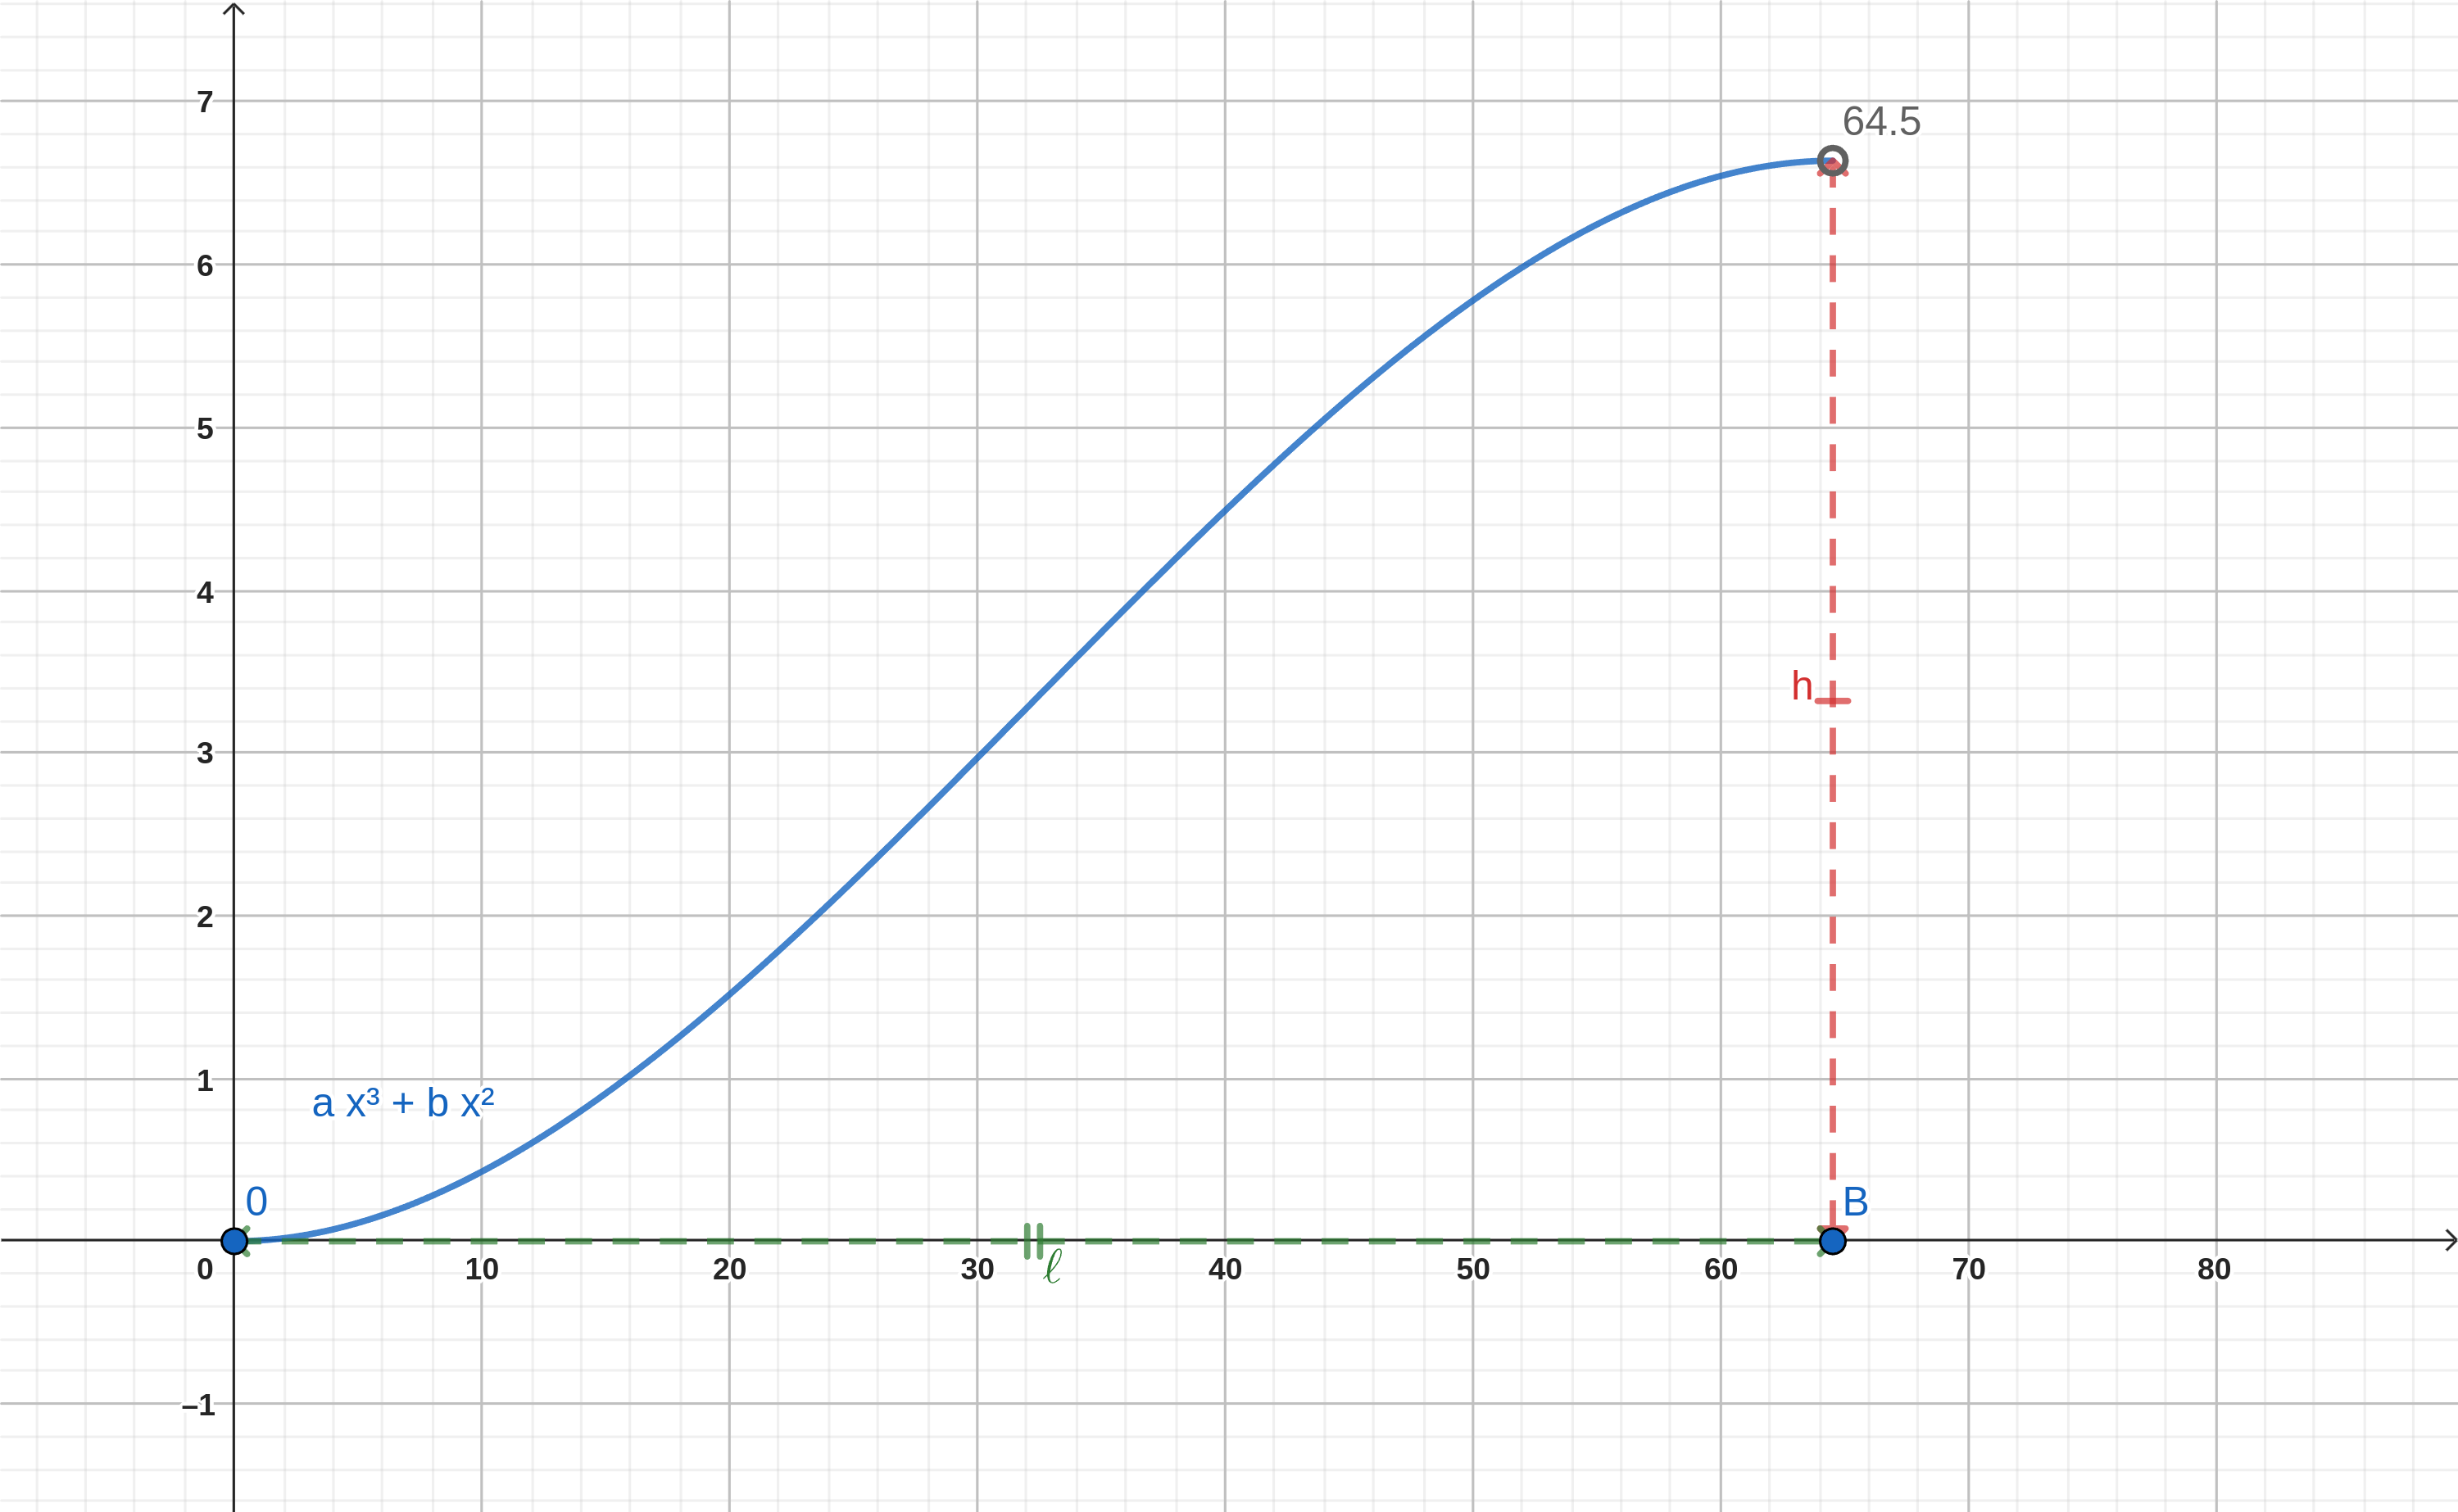
\includegraphics[height = 0.4\textheight]{recursos/geogebra-export-piloto.png}
\end{figure}
\chapter*{STEWART SECCION 3.5 EJERCICIO 80}
1. \textbf{Ecuación de la elipse:}
\[
x^2 + 4y^2 = 5
\]

2. \textbf{Derivada implícita de la elipse respecto a \(x\):}
\[
\frac{d}{dx}(x^2 + 4y^2) = \frac{dy}{dx}(5)
\]
\[
2x + 8y\frac{d}{dx} = 0
\]

3. \textbf{Despeje de \( \frac{d}{dx} \):}

\[
\frac{d}{dx} = -\frac{x}{4y}
\]

4. \textbf{Sustitución del punto \((-5, 0)\) en la fórmula de la pendiente:}
\[
\frac{d}{dx} = -\frac{-5}{4(0)} = \infty
\]

5. \textbf{Ecuación de la recta que conecta los puntos \((-5, 0)\) y \((3, h)\):}
\[
\text{Pendiente} = \frac{h - 0}{3 - (-5)} = \frac{h}{8}
\]

6. \textbf{Igualación de la pendiente de la recta con la pendiente de la tangente:}
\[
\frac{h}{8}
\]

7. \textbf{Por lo tanto \(h\):}
\[
\frac{h}{8} 
\]


\chapter*{ ANTON-BIVENS-DAVIS 3.1 EJERCICIO 40}

\textbf{39-40:} Se dice que dos curvas son \textbf{ortogonales} si sus líneas tangentes son perpendiculares en cada punto de intersección, y dos familias de curvas son \textbf{trayectorias ortogonales} una de otra, si cada miembro de la familia, es ortogonal de otro miembro de la otra familia. Esta terminología es usada en estos ejercicios. \newline

\textbf{40.} La figura muestra algunos miembros típicos de la familia de hiperbolas $xy = c$ (curvas negras) y $x^{2} - y^{2} = k$ (curvas grises), donde $ c \neq 0$ y $ k \neq 0$. Usar la pista de 39 para mostrar que estas familias son trayectorias ortogonales una de otra. [*HINT 39: Para que las rectas tangentes sean perpendiculares en un punto de la intersección, las pendientes de esas rectas tangentes deber ser recíprocas negativas una de otra]. \\
\newline
\begin{center}
    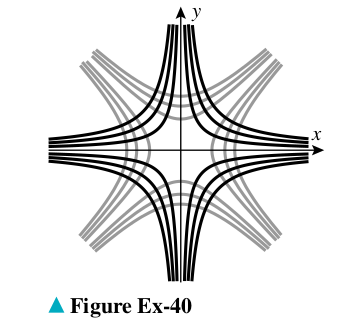
\includegraphics[height = 0.25\textheight]{recursos/Grafo40.png}\par
\end{center}

\textbf{Desarrollo:}\newline
Se debe mostrar que para cada miembro de la familia $xy = c$ hay una curva ortogonal a ella en la familia  $x^{2} - y^{2} = k$ . \\
Para esto las pendientes de estas dos curvas deber ser el recíproco negativo de la otra pendiente. (La pendiente de la recta tangente en un punto es la derivada).\\
\newline
\textbf{1) Derivar:} Derivar las ecuaciones de cada familia, tomando a $c$ y $k$ como constantes. (Derivación implícita).
\begin{align*}
   xy &= c           &... (1)\\
   x^{2} - y^{2} &= k              &...(2)
\end{align*}
\newline
\textbf{Derivando (1):}
\begin{align*}
    \frac{d}{dx}xy &= \frac{d}{dx}c \\
    \frac{d}{dx}xy &= 0 \\
    x\frac{d}{dx}y  +  y\frac{d}{dx}x &= 0 \\
    x\frac{dy}{dx} +  y(1) &= 0 \\
    x\frac{dy}{dx}  &= -y \\
    \frac{dy}{dx}  &= -\frac{y}{x}\\
    m_{1}  &= -\frac{y}{x}
\end{align*}
\newline
\textbf{Derivando (2):}
\begin{align*}
    \frac{d}{dx}(x^{2} - y^{2}) &= \frac{d}{dx}k \\
    \frac{d}{dx}x^{2} -  \frac{d}{dx}y^{2} &= 0\\
    2x -  2y\frac{d}{dx}y &= 0\\
    -2y\frac{dy}{dx} &= -2x\\
    \frac{dy}{dx} &= \frac{-2x}{-2y}\\
    \frac{dy}{dx} &= \frac{x}{y}\\
    m_{2}  &= \frac{x}{y}
\end{align*}
\newline
\textbf{Ahora} teniendo ambas pendientes, el recíproco negativo de una debe ser la otra. \\
\begin{center}
    $ m_{1}  = -\frac{1}{m_{2}}$      y    $ m_{2}  = -\frac{1}{m_{1}}$\\
\end{center}
\textbf{Entonces:}
\begin{center}
    Si $ m_{1}  = -\frac{y}{x} $ \\
    $\Rightarrow$ 
\end{center}
\begin{align*}
   -\frac{1}{m_{1}} &= -\frac{1}{-\frac{y}{x}}\\
   -\frac{1}{m_{1}} &= -\frac{\frac{1}{1}}{-\frac{y}{x}}\\
   -\frac{1}{m_{1}} &= -\frac{1(x)}{1(-y)}\\
   -\frac{1}{m_{1}} &= -\frac{x}{-y}\\
   -\frac{1}{m_{1}} &= \frac{x}{y}\\
\end{align*}
\[
  -\frac{1}{m_{1}} = \frac{x}{y} = m_{2}
\]
\[
\therefore  m_{1}  = -\frac{1}{m_{2}}   \Leftrightarrow   m_{2}  = -\frac{1}{m_{1}}
\]
\newline
Ambas pendientes son la recíproca negativa de la otra. Así podemos decir que estas familias de curvas son trayectorias ortogonales.
\chapter*{STEWART SECCION 3.7 EJERCICIO 16}
El volumen de una célula esférica en crecimiento es $V=\frac{4}{3}\pi r^3$, donde el radio $r$ se mide en micrómetros ($1\;\mu m = 10^{-6}m$).
\begin{enumerate}[label=\alph*)]
	\item Encuentre la razón de combio promedio de $V$ respecto a $r$, cuando este cambia de
	      \begin{multicols}{6}
		      \noindent
		      \begin{enumerate}[label=\roman*)]
			      \item 5 a 8 $\mu m$
			            \columnbreak
			      \item 5 a 6 $\mu m$
			            \columnbreak
			      \item 5 a 5.1 $\mu m$
		      \end{enumerate}
	      \end{multicols}
	\item Halle la razón de cambio instantánea de $V$ respecto a $r$, cuando $r=5\mu m$
	\item Demuestra que la razón de cambio del volumen de una esfera respecto a su radio es igual a su área superficial.
	      Explique geométricamente por qué esto es cierto.
\end{enumerate}

\textbf{Inciso a)} Con base en que la razón de cambio de $y$ respecto de $x$ en el intervalo $[x_1,  x_2]$ puede interpretarse como la pendiente de la recta secante, esot es el cociente de diferencias $$\frac{\Delta y}{\Delta x}=\frac{f(x_2)-f(x_1)}{x_2-x_1}$$
Para este caso, nuestra función del Volumen que depende del radio $$V(r)=\frac{4}{3}\pi r^3$$. Para saber la razón de cambio promedio es necesario efectuar el razonamiento anterior, dado:$$\frac{\Delta V}{\Delta r}=\frac{V(r_1)-V(r_2)}{r_1-r_2}$$
para
\begin{multicols}{6}
	\noindent
	\begin{enumerate}[label=\roman*)]
		\item $r_1=5$ a $r_2=8$ $\mu m$
		      \columnbreak
		\item $r_1=5$ a $r_2=6$ $\mu m$
		      \columnbreak
		\item $r_1=5$ a $r_2=5.1$ $\mu m$
	\end{enumerate}
\end{multicols}
$\therefore \text{Sustituyendo en la ecuación}$
\begin{multicols*}{3}
	\noindent
	\begin{align*}
		\implies I)\; \frac{\Delta V}{\Delta r} = & \frac{V(8)-V(5)}{8-5}                               \\
		\implies\frac{\Delta V}{\Delta r} =       & \frac{\frac{4}{3}\pi(8)^3-\frac{4}{3}\pi(5)^3}{8-5} \\
        =       & \frac{\frac{4}{3}\pi(8^3-5^3)}{3}\\
        =       &\frac{\frac{4}{3}\pi(512-125)}{3}\\
        =       &\frac{\frac{4}{3}\pi(387)}{3}\\
        =       &\frac{4}{9}\pi(387)\\
		\simeq                                    & 540.3539 \; \mu m^3/\mu m
	\end{align*}
	\columnbreak
	\begin{align*}
		\implies II)\; \frac{\Delta V}{\Delta r} = & \frac{V(6)-V(5)}{6-5}                               \\
		\implies\frac{\Delta V}{\Delta r} =        & \frac{\frac{4}{3}\pi(6)^3-\frac{4}{3}\pi(5)^3}{6-5} \\
		=                                          & \frac{\frac{4}{3}\pi((6)^3-(5)^3)}{1}               \\
		=                                          & \frac{4}{3}\pi((6)^3-(5)^3)                         \\
		=                                          & \frac{4}{3}\pi(91)                                  \\
		\simeq                                     & 381.1800\; \mu m^3/\mu m                                    \\
	\end{align*}
	\columnbreak
	\begin{align*}
		\implies III)\; \frac{\Delta V}{\Delta r} = & \frac{V(5.1)-V(5)}{5.1-5}                               \\
		\implies \frac{\Delta V}{\Delta r} =        & \frac{\frac{4}{3}\pi(5.1)^3-\frac{4}{3}\pi(5)^3}{5.1-5} \\
		=                                           & \frac{\frac{4}{3}\pi((5.1)^3-(5)^3)}{0.1}               \\
		=                                           & \frac{4\pi(7.651)}{3\cdot 0.1}                          \\
		=                                           & \frac{4}{0.3}\cdot \pi(7.651)                           \\
		\simeq                                      & 320.4843\;\mu m^3/\mu m
	\end{align*}
\end{multicols*}
$\therefore$ Las razones medias de coambio para los valores de I), II) y III) respectivamente son
$$I)\simeq 810.5310 \; \mu m$$
$$II)\simeq 381.1800\; \mu m$$
$$III)\simeq 320.4843\;\mu m$$
\textbf{Inciso b)} Su límite, cuando $\Delta x \rightarrow 0$ es la derivada $f'(x_1)$, la cual puede interpretarse como la razón de cambio instantánea de y respecto a x, o sea, la pendiente de la recta tangente en $P(x_1, f(x_1))$.
Dicho esto la derivada de $V(r)$ es la razón de coambio instantánea: $$\therefore \left.\frac{dV}{dr}\right|_{r=5\;\mu m}=\left . 4\pi r^2\right|_{r=5\;\mu m}$$
$$\implies 4\pi (5)^2\simeq 314.1592 \;\mu m^3/\mu m$$

\textbf{Inciso c)} Ciertamente definimos que el volumen de la célula (nuestra esfera) está dado por $$V=\frac{4}{3}\pi r^3$$
La razón de cambio del volumen respecto a radio es la derivada de V $$\frac{dV}{dr}=4\pi r^2$$

De este modo, si el incremendo del radio es un pequeño intervalo  dr, estonces el cambio del volumen de la esfera $(dV)$ se puede aproximar como la "capa" adicional de volumen que se añade a la superficie de la esfera inicial
$$\Delta V \approx 4\pi r^2 \cdot \Delta r$$
Al dividir por $\Delta r$ , obtenemos:$$\frac{\Delta V}{\Delta r} \approx 4\pi r^2$$

Por lo tanto, la razón de cambio del volumen de una esfera respecto a su radio es igual a su área superficial, de manera similar a cómo la razón de cambio del area del circulo es aproximadamente igual a la circunferencia por el incremento del radio.


\chapter*{STEWART SECCION 3.7 EJERCICIO 19}

\textbf{19.} La cantidad de carga, $Q$, en coulombs $c)$ que ha pasado por un punto de un alambre hasta el tiempo $t$ (medidio en segundos) se expresa con $Q(t) = t^{3} - 2t_{2} + 6t +2$. Encuentre la corriente cuando $ a) t = 0.5s$ y $b) t = 1s$ [Véase el ejemplo 3. La unidad de corriente es el ampere ($1A = 1C/s$).] ¿En qué momento la corriente es la más baja?\\
\newline
\textbf{Desarrollo:}\newline
De acuerdo al ejemplo 3, la corriente es la rapidez con que la carga fluye por una suerficie. (C/s) = A.\\
\newline
$\Delta Q$ es la carga y $\Delta t$ es el periodo de tiempo. La corriente promedio en un intervalo de tiempo se da por $\frac{\Delta Q}{\Delta t}$, tomando el límite de la corriente en lapsos de tiempo muy pequeños $\Delta t \rightarrow 0$, obtenemos a lo que llamamos la corriente $I$ en un instante dado $t_{1}$.\\
\newline
\[
I = \lim_{\Delta t \to 0 }{\frac{\Delta Q}{\Delta t}} = \frac{dQ}{dt}
\] \\
la corriente es la derivada de la carga.\\
\newline
\textbf{Carga en Función del tiempo:}
\[
Q(t) = t^{3} - 2t^{2} + 6t + 2 
\]
\textbf{Derivar: }Derivando $Q(t)$ para obtener función de corriente.
\begin{align*}
    \frac{d}{dt}Q(t) &= \frac{d}{dt}(t^{3}-2t^{2}+6t+2)\\
    \frac{dQ}{dt} &= \frac{d}{dt}t^{3} - \frac{d}{dt}2t^{2} + \frac{d}{dt}6t + \frac{d}{dt}2\\
    \frac{dQ}{dt} &= 3t^{2} - 4t +6\\
    I &= 3t^{2} - 4t +6\\
\end{align*}
\textbf{Evaluando en los tiempos dados:}\\
\newline
\textbf{a)} $t = 0.5 s$
\begin{align*}
    I(0.5) &= 3(0.5)^{2} - 4(0.5) +6\\
    I(0.5) &= 3(0.25) - 4(0.5) +6\\
    I(0.5) &= 0.75 - 2 +6\\
    I(0.5) &= 4.75 A\\
\end{align*}
\textbf{b)} $t = 1 s$
\begin{align*}
    I(1) &= 3(1)^{2} - 4(1) +6\\
    I(1) &= 3(1) - 4 +6\\
    I(1) &= 3 - 4 +6\\
    I(1) &= 5 A\\
\end{align*}
\textbf{¿En qué momento la corriente es la más baja?}
\[
I(t_{min}) = I_{min}
\]
Primero, derivar la función $I(t)$.
\begin{align*}
    \frac{d}{dt}I(t) &= \frac{d}{dt}(3t^{2} -  +6)\\
    \frac{dI}{dt} &= \frac{d}{dt}3t^{2} - \frac{d}{dt}4t + \frac{d}{dt}6\\
    \frac{dI}{dt} &= 6t -4\\
\end{align*}
Resolver $\frac{dI}{dt} = 0$
\begin{align*}
    \frac{d}{dt}I(t) &= 0\\
    6t -4 &= 0\\
    6t &= 4\\
    t &= \frac{4}{6}\\
    t &= \frac{2}{3}\\
    t_{min} &= \frac{2}{3}\\
\end{align*}
Dado que en este punto la corriente presenta un mínimo es la más baja.
\chapter*{STEWART SECCION 3.7 EJERCICIO 21}
\section*{Demostración}

1. Definición de la fuerza como la derivada del momentum:
\[
F = \frac{d}{dt}(mv)
\]

2. Momentum relativista:
\[
p = mv = \frac{m_0 v}{\sqrt{1 - \frac{v^2}{c^2}}}
\]

3. Masa relativista:
\[
m = \frac{m_0}{\sqrt{1 - \frac{v^2}{c^2}}}
\]

4. Derivada del momentum relativista:
\[
F = \frac{d}{dt} \left( \frac{m_0 v}{\sqrt{1 - \frac{v^2}{c^2}}} \right)
\]

5. Aplicando la regla del producto:
\[
F = m_0 \frac{d}{dt} \left( \frac{v}{\sqrt{1 - \frac{v^2}{c^2}}} \right)
\]

6. Derivada del primer término:
\[
F = m_0 \left[ \frac{d}{dt}(v) \cdot \frac{1}{\sqrt{1 - \frac{v^2}{c^2}}} + v \cdot \frac{d}{dt}\left( \frac{1}{\sqrt{1 - \frac{v^2}{c^2}}} \right) \right]
\]

7. Primera derivada: 
\[
F = m_0 \left[ \frac{a}{\sqrt{1 - \frac{v^2}{c^2}}} + v \cdot \frac{d}{dt}\left( \frac{1}{\sqrt{1 - \frac{v^2}{c^2}}} \right) \right]
\]

8. Derivada del segundo término usando la regla de la cadena:
\[
\frac{d}{dt}\left( \frac{1}{\sqrt{1 - \frac{v^2}{c^2}}} \right) = \frac{\frac{v}{c^2}}{\left(1 - \frac{v^2}{c^2}\right)^{3/2}} \cdot \frac{dv}{dt}
\]

9. Sustitución de \( \frac{dv}{dt} = a \):
\[
\frac{d}{dt}\left( \frac{1}{\sqrt{1 - \frac{v^2}{c^2}}} \right) = \frac{v a}{c^2 \left(1 - \frac{v^2}{c^2}\right)^{3/2}}
\]

10. Sustitución en la fuerza:
\[
F = m_0 \left[ \frac{a}{\sqrt{1 - \frac{v^2}{c^2}}} + v \cdot \frac{v a}{c^2 \left(1 - \frac{v^2}{c^2}\right)^{3/2}} \right]
\]

11. Factor común de \( a \):
\[
F = m_0 a \left[ \frac{1}{\sqrt{1 - \frac{v^2}{c^2}}} + \frac{v^2}{c^2 \left(1 - \frac{v^2}{c^2}\right)^{3/2}} \right]
\]

12. Suma de los términos:
\[
F = m_0 a \left[ \frac{1 \cdot \left(1 - \frac{v^2}{c^2}\right) + \frac{v^2}{c^2}}{\left(1 - \frac{v^2}{c^2}\right)^{3/2}} \right]
\]

13. Simplificando:
\[
F = m_0 a \left[ \frac{1 - \frac{v^2}{c^2} + \frac{v^2}{c^2}}{\left(1 - \frac{v^2}{c^2}\right)^{3/2}} \right]
\]

14. Simplificando:
\[
F = m_0 a \left[ \frac{1}{\left(1 - \frac{v^2}{c^2}\right)^{3/2}} \right]
\]

15. Simplificando:
\[
F = \frac{m_0 a}{\left(1 - \frac{v^2}{c^2}\right)^{3/2}}
\]

16. Expresión final de la fuerza relativista:
\[
F = \frac{m_0 a}{\left(1 - \frac{v^2}{c^2}\right)^{3/2}}
\]


\end{document}